\chapter{Results}\label{ch5}
In the previous chapters, we have introduced the concept of the \acrlong{v2dm}.
In \Cref{ch2}, a necessary set of $N$-representability conditions were derived and in \Cref{ch3} we have shown the computational methods
that can be used to do the actual optimization.
It is time to use this knowledge. First we look into \gls{doci} and explain the motivation for the \gls{doci} $N$-representability conditions derived in \Cref{ch2-doci}.
Next, we explore orbital optimization with the goal to combine it with \gls{v2dm} restricted to \gls{doci}. We then try our method on several
benchmark systems to assess its merits.

\section{Introduction}\label{ch5-doci-intro}

Before we begin the story of the marriage between \gls{doci} and \gls{v2dm}, let us take a step back and consider the origins of
\gls{doci}. First we will introduce some classic concepts of wavefunction-based methods \citep{helgaker2007molecular}.

\begin{figure}
    \captionsetup{justification=centering}
    \begin{subfigure}[b]{0.5\textwidth}
        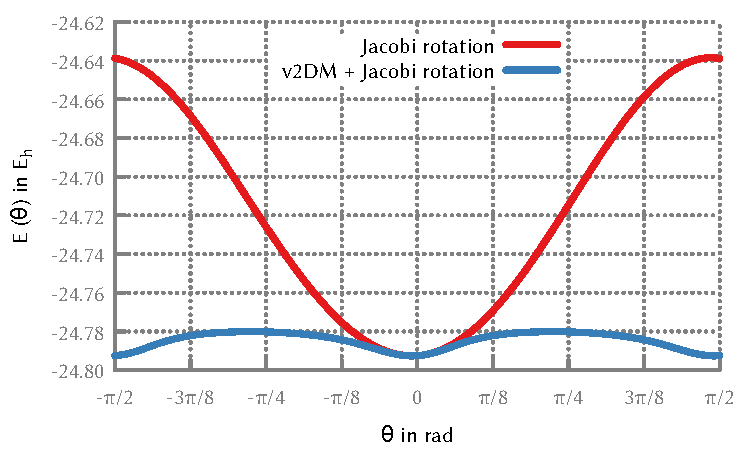
\includegraphics[width=\textwidth]{BH/orbs-scan-0-1.pdf}
        \caption{Orbitals $1A_1$ and $2A_1$,\\ min $\approx$ -0.027 rad}
        \label{5-fig3-01}
    \end{subfigure}
    \quad
    \begin{subfigure}[b]{0.5\textwidth}
        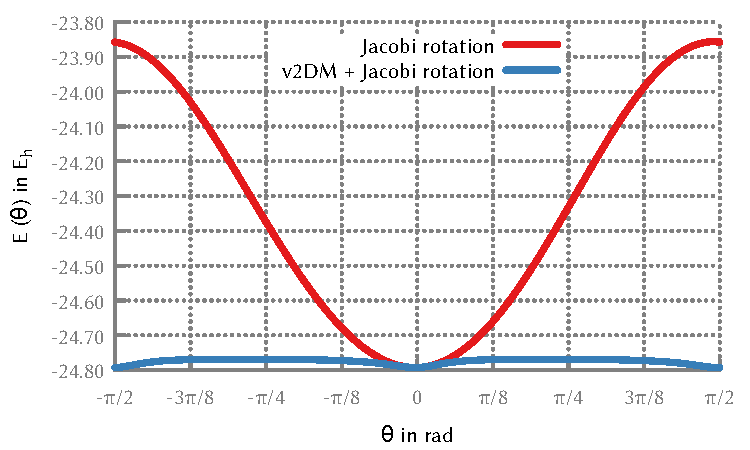
\includegraphics[width=\textwidth]{BH/orbs-scan-0-2.pdf}
        \caption{Orbitals $1A_1$ and $3A_1$,\\ min $\approx$ -0.011 rad}
        \label{5-fig3-02}
    \end{subfigure}
    \begin{subfigure}[b]{0.5\textwidth}
        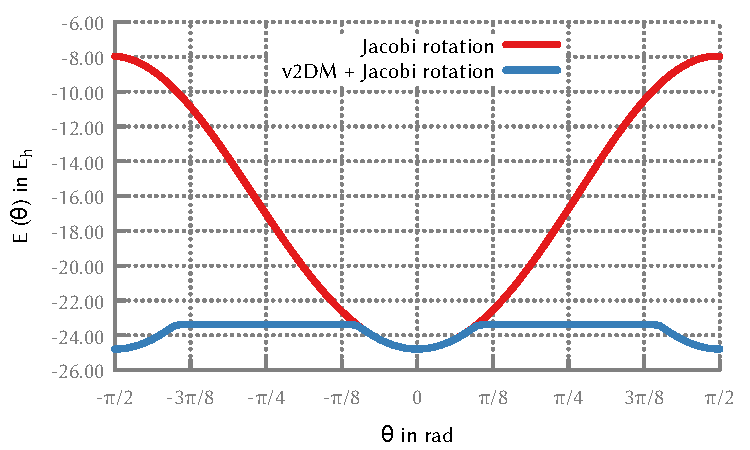
\includegraphics[width=\textwidth]{BH/orbs-scan-0-3.pdf}
        \caption{Orbitals $1A_1$ and $4A_1$,\\ min $\approx$ 0.000 rad}
        \label{5-fig3-03}
    \end{subfigure}
    \quad
    \begin{subfigure}[b]{0.5\textwidth}
        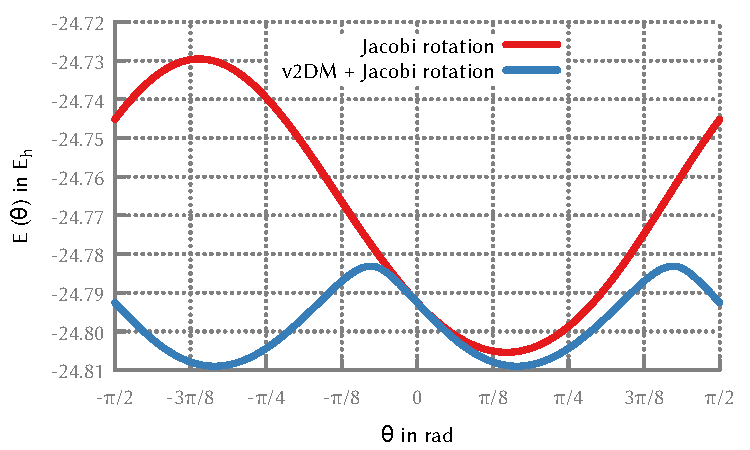
\includegraphics[width=\textwidth]{BH/orbs-scan-1-2.pdf}
        \caption{Orbitals $2A_1$ and $3A_1$,\\ min $\approx$ 0.463 rad}
        \label{5-fig3-12}
    \end{subfigure}
    \begin{subfigure}[b]{0.5\textwidth}
        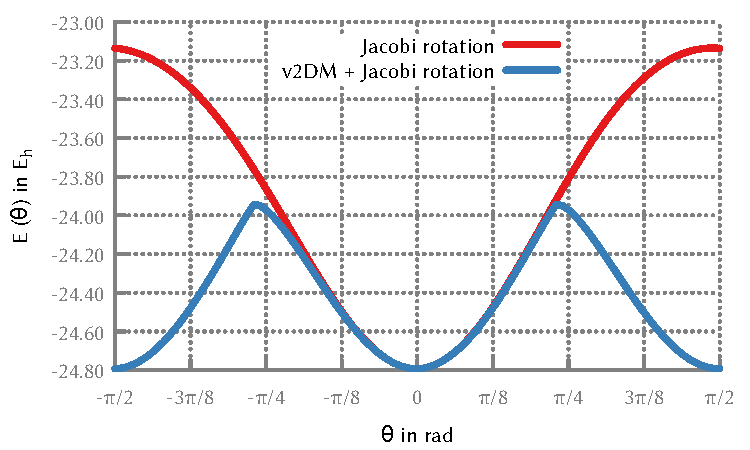
\includegraphics[width=\textwidth]{BH/orbs-scan-1-3.pdf}
        \caption{Orbitals $2A_1$ and $4A_1$,\\ min $\approx$ -0.005 rad}
        \label{5-fig3-13}
    \end{subfigure}
    \quad
    \begin{subfigure}[b]{0.5\textwidth}
        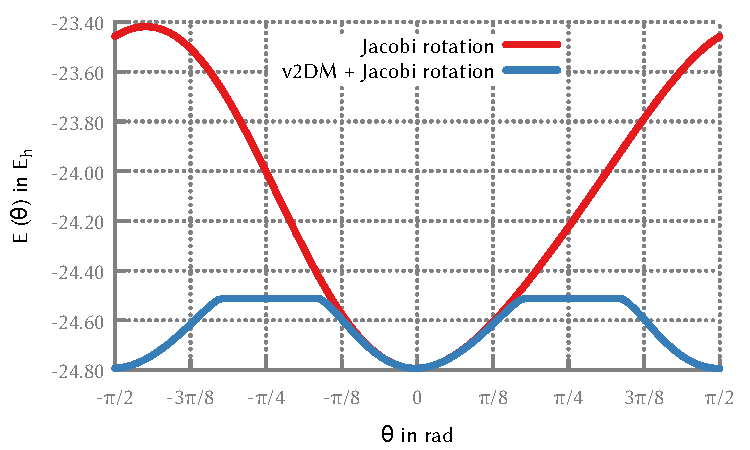
\includegraphics[width=\textwidth]{BH/orbs-scan-2-3.pdf}
        \caption{Orbitals $3A_1$ and $4A_1$,\\ min $\approx$ -0.010 rad}
        \label{5-fig3-23}
    \end{subfigure}
    \captionsetup{justification=raggedright}
    \caption{The red curve has been calculated using XX, while the dashed blue curve uses the same transformed reduced Hamiltonian but an optimized 2DM. The min refers to the minimum of the red curve. The \gls{fullci} energy is \mbox{-24.810 E$_\text{h}$}.}
    \label{5-fig3}
\end{figure}


% vim: syntax=tex spell spelllang=en tw=130 
